\chapter{Features und Merkmale}\label{chab:FeaturesundMerkmale}
\thispagestyle{standard}
\pagestyle{standard}
\renewcommand{\footrulewidth}{0.4pt}
\lfoot{\small Refik Kerimi}
In diesem Kapitel werden die Komponenten der \acl{PWA} (\acs{PWA}) erklärt. Weiters werden durch die folgenden Tabellen die wichtigsten Punkte zwischen den verschiedenen Technologien  gegenübergestellt.

\section{Aufbau Progressive Web Apps (PWA)}
Die \acs{PWA}s sind keine neuen Technologien, vielmehr sind es verbesserte Stategien, Methoden und APIs wie in Abbildung \ref{fig:Komponenten} zu sehen. 
Sie erleichtern dem User die Benutzung und den Zugriff einer \acs{Web-App} \cite{AlternativePWA}. 

\begin{figure}[h]
	\centering
	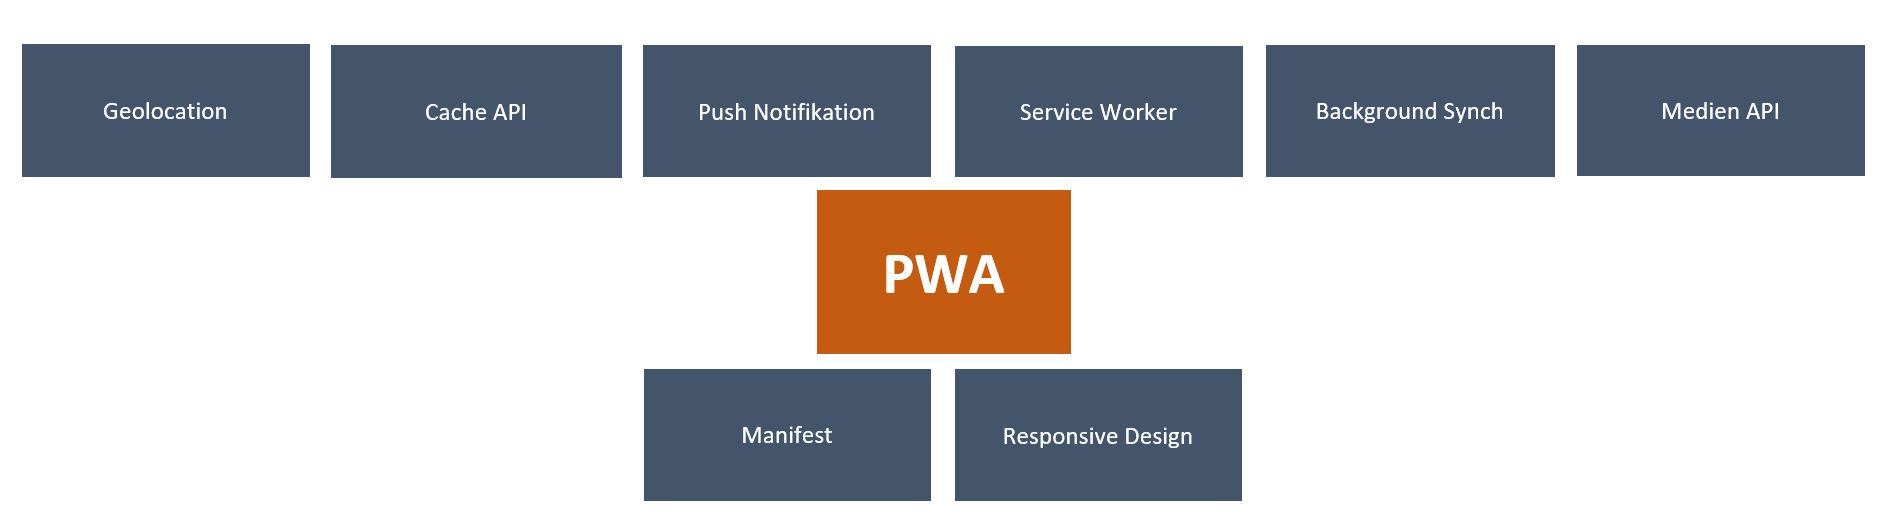
\includegraphics[width=14cm]{BilderAllgemein/PWA_Features}\medskip
	\caption{PWA Komponenten}
	\label{fig:Komponenten}
\end{figure}

\section{Unterschiede PWA, Native Applikation und Web-Apps}\label{chap:UnterschiedePWA,NativeApplikationundWeb-Apps}
In den folgenden Tabellen \ref{tab:PwaNvaWaInstallation}, \ref{tab:PwaNvaWaZugriff} und \ref{tab:PwaNvaWaFunktionen}  wird versucht die Features und Merkmale gegenüberzustellen um die Auswahl zu erleichtern. Die Unterschiede in den Punkten Veröffentlichung, Installation, Zugriff und Funktionen werden verglichen.

%Folgende Punkte werden verglichen:
%\begin{itemize}
%    \item  \textbf{Veröffentlichung und Installation}
%	\item  \textbf{Zugriff}
%	\item  \textbf{Funktionen}
%\end{itemize}. 

\begin{table}[h]
\centering

\begin{tabular} {|p{3cm}|p{3.5cm}|p{3.5cm}|p{3.5cm}|}
\hline\multirow{3}{*}
 										&PWA  & Native & Web App	\\ \hline
Veröffentlichung & Es werden verschiedene Entwicklerkonten benötigt Play Store und Apple Store & keine Entwicklerkonten benötigt & keine Entwicklerkonten benötigt\\ \hline

Installation & App muss aus einem der App-Stores downgeloaded werden  & Wird mit einem Klick auf dem Startbildschirm hinzugefügt & keine Funktion\\ \hline

Updates &  über App-Store & Serverseitig & Serverseitig\\ \hline
   				  						 
				
\end{tabular}    
\caption{Veröffentlichung und Installation \cite{PwaNvaWa}}
\label{tab:PwaNvaWaInstallation}
\end{table}


\begin{table}[h]
\centering

\begin{tabular} {|p{3cm}|p{3.5cm}|p{3.5cm}|p{3.5cm}|}
\hline\multirow{3}{*}
 										&PWA  & Native & Web App	\\ \hline
Offline-Zugriff & Verfügbar & Man muss die App einmal online nutzen, dann sollten die Inhalte im Cache offline verfügbar sein. & nicht möglich\\ \hline

Starten im Vollbildmodus & Verfügbar  & Verfügbar & nicht möglich\\ \hline

Kundenbindung &  sehr hoch, Kunden verbringen viel Zeit & App ist wie ein Tap, das macht es für den Kunden leichter zu wechseln & wie \acs{PWA}\\ \hline


				  						 
				
\end{tabular}    
\caption{Zugriff \cite{PwaNvaWa}}
\label{tab:PwaNvaWaZugriff}
\end{table}

%Tabelle verwenden
%https://apptooltester.com/de/progressive-web-%apps/
%https://www.html-seminar.de/web-app-versus-native-app.htm --> native versus web app

\begin{table}[h]
\centering

\begin{tabular} {|p{3cm}|p{3.5cm}|p{3.5cm}|p{3.5cm}|}
\hline\multirow{3}{*}
 										&PWA  & Native & Web App	\\ \hline
Push-Nachrichten & Verfügbar & Verfügbar (nur für Android) & Verfügbar (mit zusätzliche Tools)\\ \hline

Geolocation & Verfügbar  & Verfügbar & Verfügbar\\ \hline

Kamera-/Mikrofonzugriff &  Verfügbar & Verfügbar & Verfügbar\\ \hline

Gerätevibration &  Verfügbar & Verfügbar & nicht Verfügbar\\ \hline

Responsive &  Verfügbar & Verfügbar & Verfügbar\\ \hline

Akkuladestatus &  Verfügbar & Verfügbar & nicht Verfügbar\\ \hline

Zugriff auf Kontakte und Kalender &  Verfügbar & nicht Verfügbar & nicht Verfügbar\\ \hline

Telefon: SMS oder Anrufe &  Verfügbar & nicht Verfügbar & nicht Verfügbar\\ \hline				  						 			
\end{tabular}    
\caption{Funktionen \cite{PwaNvaWa}}
\label{tab:PwaNvaWaFunktionen}
\end{table}
\newpage
\clearpage

Wie in den Tabellen ersichtlich bietet die \acs{PWA} eine Reihe von Vorteilen, z.B. Push Notifikations und Offline-Zugriff, die bei der Benutzung behilflich sein können. Aufgrund dessen bietet sie eine gute Alternative zu den Native App. Probleme machen die Betriebssysteme, da nicht alle Funktionen auf den verschiedenen Systemen zur Verfügung stehen \cite{PwaNvaWa}.
In den nächsten Kapiteln werden die Methoden und APIs in der Theorie und im Kapitel \ref{chap:Implementierung} die praktische Anwendung an einer selbst erstellten App erklärt. 

\section{Web App Manifest}\label{sub:Manifest}
Das App Manifest ist eine JSON Datei die dem Browser verrät, wie sich die \acs{Web-App} bei der Installation auf dem Startbildschirm verhält. Im Manifest werden der Name, der Kurzname, die Größe, das Aussehen der Icons und weitere Eigenschaften definiert. Dessen Zweck ist es der Anwendung auf dem Startbildschirm ihr Aussehen zu verleihen. 
Das App Manifest.json Datei wird in die gleiche Ebene wie die Index.html Datei in das Projekt eingepflegt und über den folgenden Link-Tag im Header implementiert: 

\begin{lstlisting}[language=HTML, caption={Manifest.json} {\cite{Manifest}},label=lst:Manifest.json, xleftmargin=50pt]
<link rel="manifest" href="/<Dateinname>">
\end{lstlisting}

Bei Anwendungen mit mehreren \acs{HTML}-Seiten muss der Link-Tag auf jeder Seite eingefügt werden. 
Im Listening \ref{lst:Manifest.jsonBsp} ist ein Auszug vom Aufbau dargestellt:
	\begin{lstlisting}[language=json, firstnumber=1, caption={Manifest in das Projekt implementieren} {\cite{Manifest}},label=lst:Manifest.jsonBsp, xleftmargin=50pt]
  "name":"PWA Smart Home RMJ",
  "short_name":"PWA_SHL_RMJ",
  "start_url":"./",
  "scope":".",
  "display":"standalone",
  "background_color":"#003399",
  "theme_color":"#3F51C5",
  "icons":[
    {
      "src":"./static/img/light48.png",
      "type":"image/png",
      "sizes":"48x48"
    }
  ]

\end{lstlisting}

Im Grunde sind alle Key Value Paare selbst erklärend und auch auf https://developers.google.com/web/fundamentals/web-app-manifest/ sehr gut beschrieben \cite{Manifest}. 

\section{Add to Homescreen}\label{sub:AddtoHomescreen}
Diese Funktion erleichtert es den Benutzern die App auf dem Desktop oder Startbildschirms zu installieren. Nach der Installation wird die PWA zum launcher hinzugefügt und wie alle anderen installierten Apps ausgeführt.
Um den Banner auf dem mobilen Gerät anzuzeigen, müssen folgende Kriterien erfüllt werden \cite{AddToHomescreen}.


\begin{itemize}
    \item  die App ist noch nicht installiert
	\item  muss min 30 Sekunden lang mit der Domäne interagieren
	\item  beinhaltet ein Web App Manifest mit folgenden Werten:
		 \begin{itemize}
         \item Kurzname oder Name
         \item icons - muss ein 192px und ein 512px großes Icon enthalten
         \item Startadresse
         \item Anzeige muss eines der folgenden sein: fullscreen, standalone oder \\ minimal-ui
      	\end{itemize}
    \item 	darf nur über HTTPS aufrufbar sein
    \item beinhaltet einen Service Worker mit einem Fetch-Event-Handler  
\end{itemize}


Nachdem die oben genannten Bedingungen erfüllt wurden, wird ein Eventlistener gestartet siehe Listing \ref{lst:beforinstallpromptEvent}


\begin{lstlisting}[language=JavaScript, caption={beforinstallpromptEvent} {\cite{AddToHomescreen}},label=lst:beforinstallpromptEvent, xleftmargin=50pt]
let deferredPrompt;

window.addEventListener('beforeinstallprompt', (e) => {
  // Prevent Chrome 67 and earlier from automatically showing the prompt
  e.preventDefault();
  // Stash the event so it can be triggered later.
  deferredPrompt = e;
});
\end{lstlisting}

In der Abbildung \ref{fig:BrowserManifest} sieht man die Browserkompabilität des Manifest Files zum Stand Juli 2018.
 
\begin{figure}[H]
	\centering
	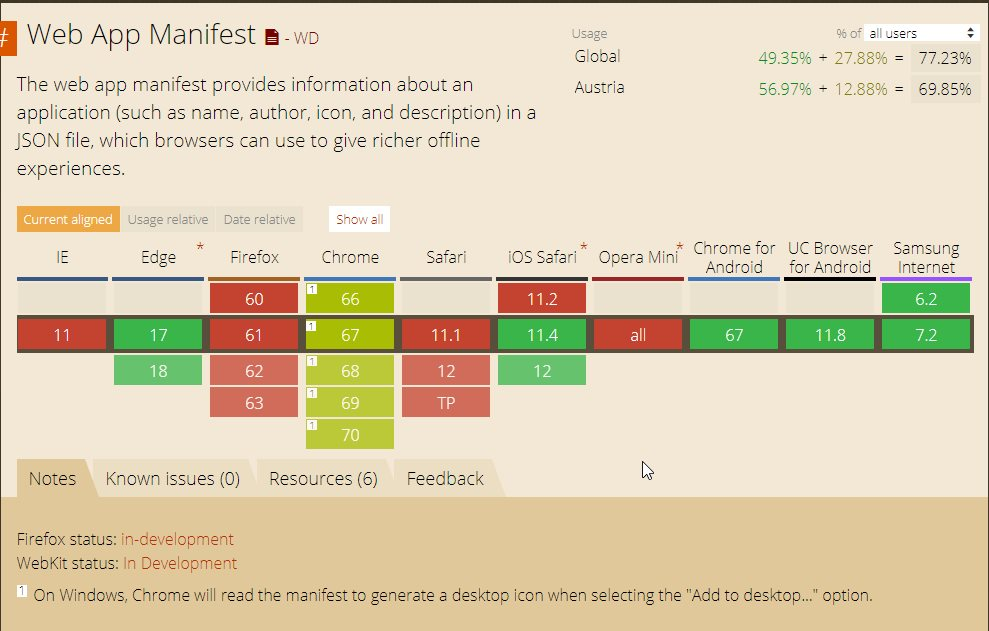
\includegraphics[width=10cm]{BilderAllgemein/BrowserManifest}\medskip
	\caption{Kompabilität Manifest.json \cite{BrowserSupport}}
	\label{fig:BrowserManifest}
\end{figure}
 


\section{Service Worker}\label{sub:ServiceWorker}
%\label{sec:Service Worker} zuweisung zu anderen Sektor
Der Server Worker ist ein Script, das vom Browser im Hintergrund ausführt \cite{ServiceWorkerRegistration}. Mit Hilfe des Server Worker ist es möglich die \acs{Web-App} offline zu betreiben, Push Notifikationen zu erhalten und gecachte Daten abzurufen. Server Worker verhalten sich wie Proxy-Server, welche in einer Zwischenschicht vom Browser und dem Netzwerk sitzen, wie in der Abbildung \ref{fig:SWProxy} zu sehen ist.

\begin{figure}[h]
	\centering
	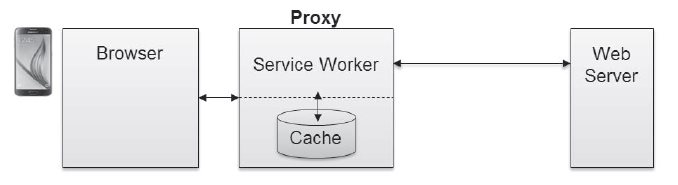
\includegraphics[width=14cm]{BilderAllgemein/SWProxy}\medskip
	\caption{Service Worker als Proxy \cite{SWProxy}}
	\label{fig:SWProxy}
\end{figure}

Ein Server Worker wird von einem Worker-Kontext ausgeführt, hat keinen DOM Zugriff und wird als Haupt-Java Script Thread verwendet \cite{Worker} \cite{ServiceWorker}.
Der komplizierteste Teil des Server Worker ist sein Lebenszyklus. 
Die Aufgabe der Lebenszyklen sind wie folgt definiert:

\begin{itemize}
    \item  Offlinverwendung
	\item  Störung eines anderen Service Workers verhindern
	\item  Stellt sicher, dass nur ein Service Worker für eine Seite zuständig ist
	\item  Stellt sicher dass nur eine Version der Webseite gleichzeitig ausgeführt wird
\end{itemize}


Der Lebenszyklus eines Server Workers ist von der Webseite getrennt.
In der Installationsphase werden die benötigten statischen Dateien zwischengespeichert und erst nach diesem Vorgang ist der Server Worker installiert. Die Installation erfolgt über die JavaScript-Funktion wie in Listing \ref{lst:ServiceWorkerNavigator}:

\begin{lstlisting}[language=JavaScript, caption={Service Worker Navigator} {\cite{ServiceWorkerRegistrationGoogle}},label=lst:ServiceWorkerNavigator, xleftmargin=50pt]
navigator.serviceWorker.register
\end{lstlisting}

Danach folgt die Aktivierungsphase. In dieser Phase werden alte Cache-Inhalte verwaltet und aktualisiert.


%\begin{figure}[h]
%	\centering
%	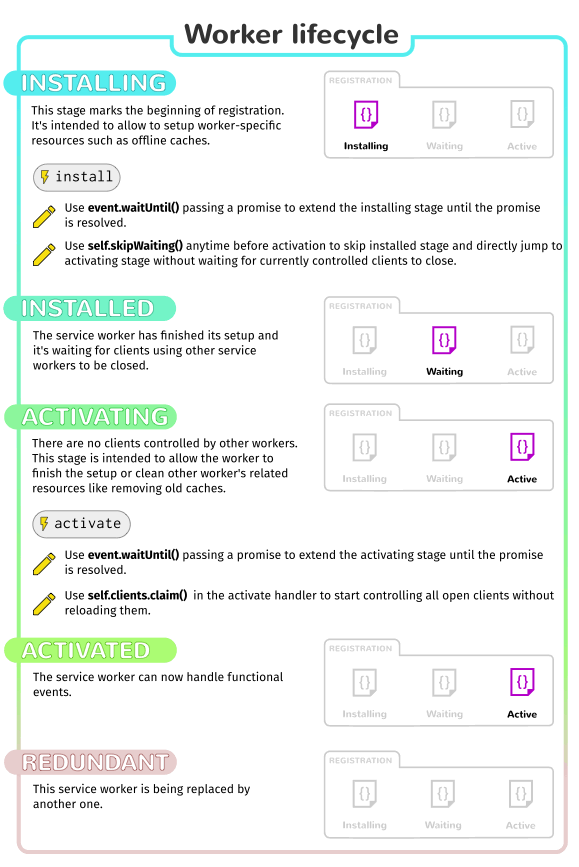
\includegraphics[width=12cm]{BilderAllgemein/swLifecycle}\medskip
%	\caption{Basis Architektur \acl{SW} \cite{ServiceWorkerArchitecture}}
%	\label{fig:Erstinstallation}
%\end{figure}


Um die neuen Seiten zu steuern muss der Server Worker erneut geladen werden.
In der Abbildung \ref{fig:Erstinstallation} ist eine vereinfachte Erstinstallation zu sehen.


Um den Service Worker zu registrieren muss folgender \acs{JS}-Code in das Projekt unter \\ \textit{/app/src/js/app.js} integriert werden.
\begin{lstlisting}[language=JavaScript, caption={Service Worker Register} {\cite{ServiceWorkerRegistration}},label=lst:ServiceWorkerRegister, xleftmargin=50pt]
if ('serviceWorker' in navigator) {
 console.log('Service Worker and Notification is supported')
    navigator.serviceWorker.register('/sw.js')
        .then(reg => {
            console.log('Service worker registered!', reg);
        })
        .catch(err => console.log(err));
  });
}
\end{lstlisting}

In Zeile eins wird im Listing \ref{lst:ServiceWorkerRegister} die Unterstützung durch den Browser geprüft, bevor in der dritten Zeile der Server Worker über die\\ \textit{navigator.serviceWorker.register('<ServiceWorker Name>')}-Funktion, wie in Abbildung \ref{fig:RegistrierungSW} zu sehen ist, aufgerufen wird.
\begin{figure}[h]
	\centering
	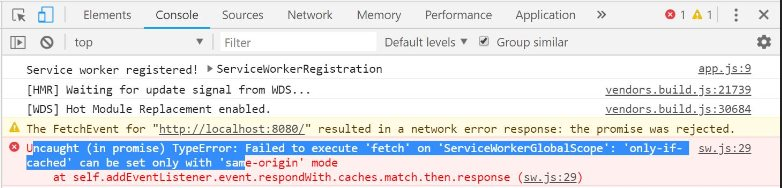
\includegraphics[width=15cm]{BilderAllgemein/SW_Registred}\medskip
	\caption{Registrierung Service Worker}
	\label{fig:RegistrierungSW}
\end{figure}

\begin{figure}[h]
	\centering
	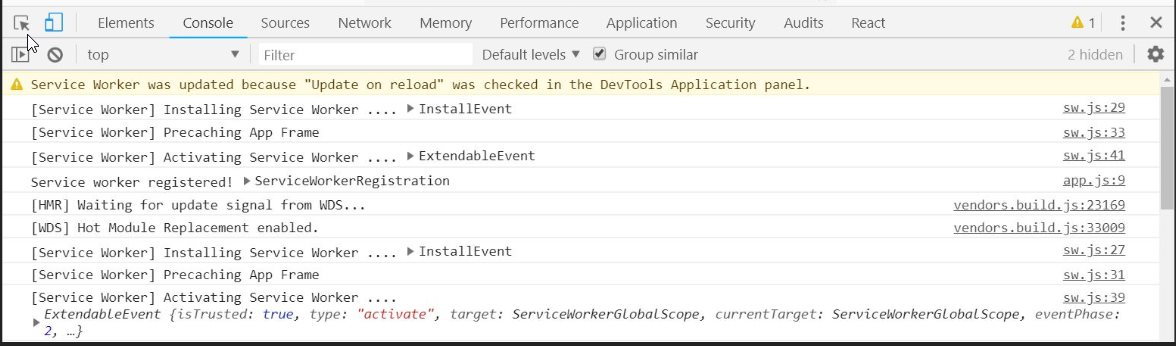
\includegraphics[width=15cm]{BilderAllgemein/SW_Activated}\medskip
	\caption{Registrierung Service Worker}
	\label{fig:Aktivierung}
\end{figure}


In der Abbildung \ref{fig:Aktivierung} ist zu sehen wie die Installation erst bei erneutem Laden der App startet. Dabei cached der Server Worker die zum Cache hinzufügten Files, bevor die Installation fertig ist.
Nach der Installation wird der Server Worker aktiviert und steht damit der Applikation zur Verfügung.


Wie in Abbildung \ref{fig:Erstinstallation} zu sehen ist kann der Server Worker nach der Übernahme der Steuerung zwei Zustände übernehmen, entweder dieser wird beendet oder er übernimmt die Verwaltung der Netzwerkanfragen und der Nachrichten \cite{ServiceWorkerRegistration}.
Die Server Worker API stellt eine Cache-Schnittstelle zum Speichern von Daten auf dem Browser, im Browsercache, zur Verfügung. Die API wurde ursprünglich für den Server Worker entwickelt, diese kann aber von jedem anderen Script verwendet werden. 
Wie die API gestaltet wird, hängt von den Anforderungen der Applikation ab.


\begin{figure}[H]
	\centering
	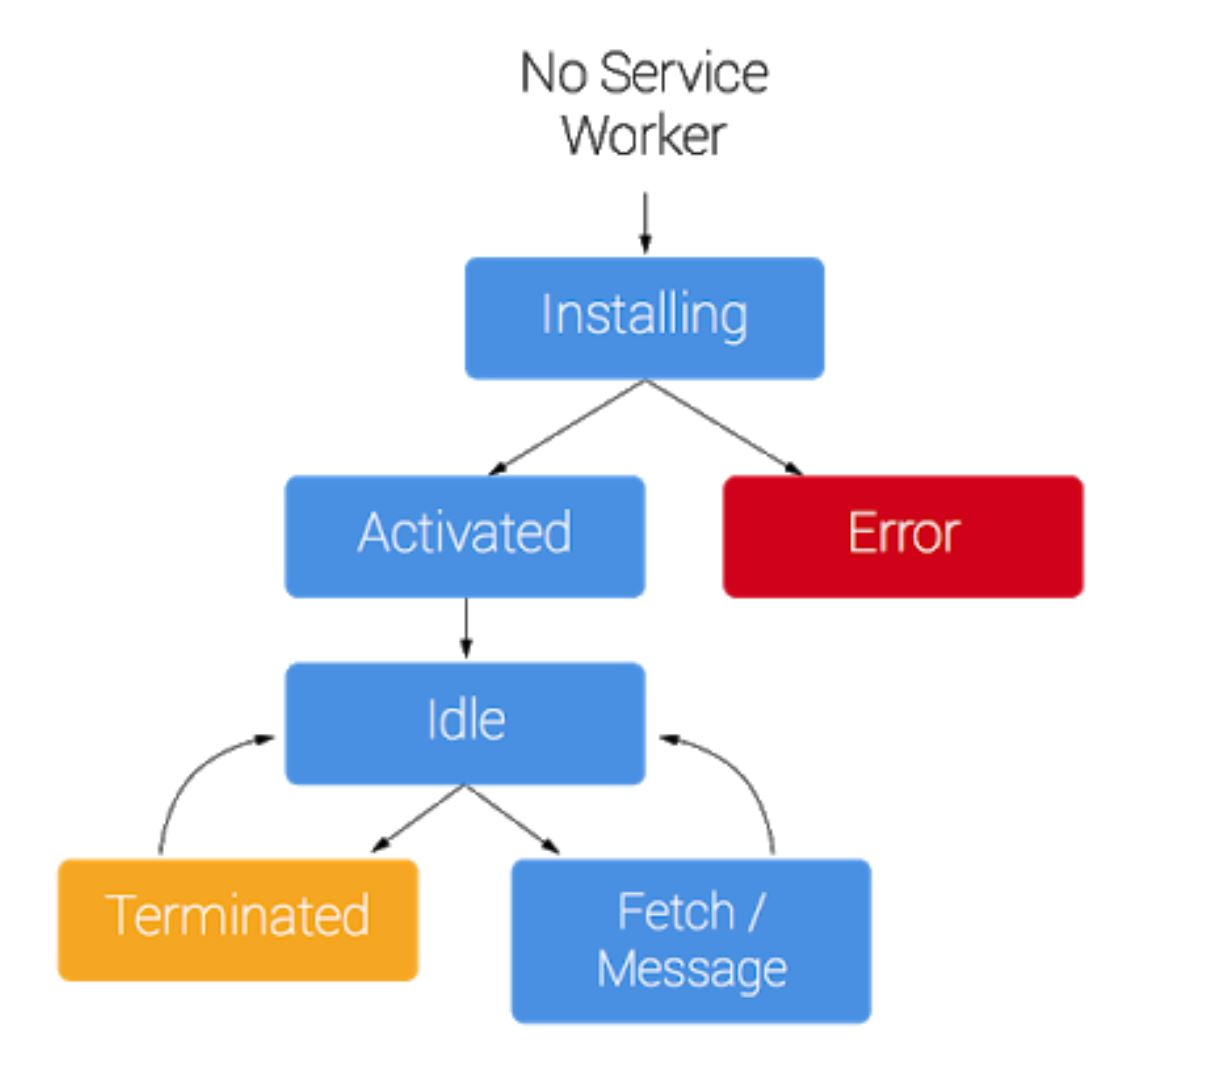
\includegraphics[width=12cm]{BilderAllgemein/InstallSW}\medskip
	\caption{Erstinstallation Service Worker \cite{ServiceWorkerRegistration}}
	\label{fig:Erstinstallation}
\end{figure}


In der Abbildung \ref{fig:BrowserSW} sieht man die Browserkompabilität des Service Workers zum Stand Juli 2018.



%https://developers.google.com/web/fundamentals/primers/service-workers/

\begin{figure}[h]
	\centering
	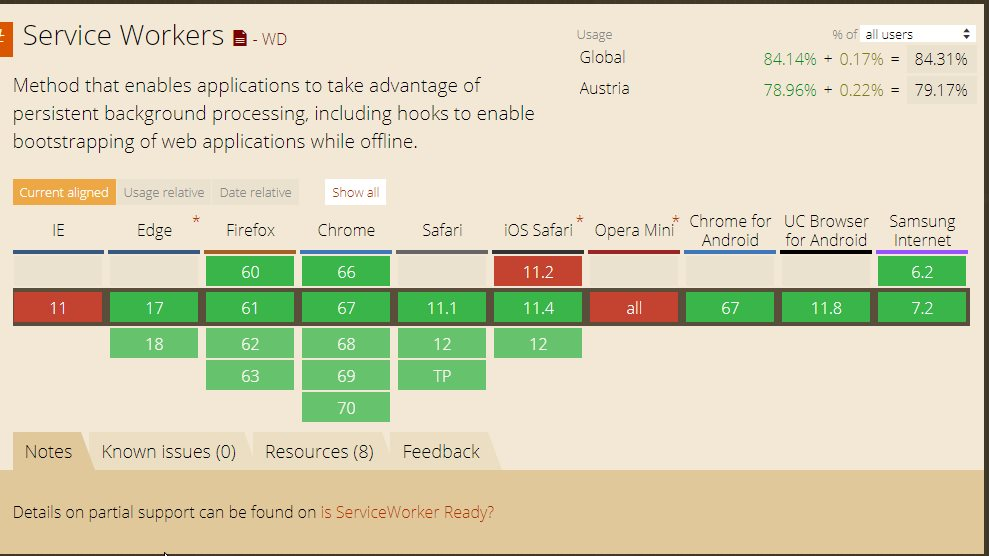
\includegraphics[width=10cm]{BilderAllgemein/BrowserSW}\medskip
	\caption{Kompabilität Service Worker \cite{BrowserSupport}}
	\label{fig:BrowserSW}
\end{figure}


\section{Push Notifikation}
Um dem User bei einer Server Worker das Gefühl von Nativen Applikationen aufkommen zu lassen ist die Push Funktion unablässig. Erst diese Funktion in Kombination mit dem Server Worker gibt den \acl{Web-App} ein individuelles Verhalten, dass bis jetzt den Native Apps vorbehalten war.
Unternehmen bekommen, durch Push APIs und Notification APIs, neue Möglichkeiten mit dem Nutzer in Kontakt zu treten und ihn mit personalisierten, relevanten Inhalten zu versorgen.
Zur Benachrichtigung oder für Push werden zwei Technologien eingesetzt. Mit Hilfe von Push werden vom Server Informationen an den Service Worker gesendet, um Informationen vom Service Worker zum Nutzer zu senden werden Benachrichtigungen verwendet. Die Technologien nutzen für diese Datenübertragung sich ergänzende APIs \cite{PushNotifikation}. \\
Im Kapitel \ref{chap:Implementierung} wird die praktische Verwendung der Benachrichtigungen genauer beschrieben.  
 

Hier wird wie in Kapitel \ref{sub:ServiceWorker} die Browserunterstützung vom Service Worker und den Push Benachrichtigungen überprüft \cite{PushNotifikation}.


In der Abbildung \ref{fig:BrowserPushAPI} sieht man die Browserkompabilität der Push API zum Stand Juli 2018.
\begin{figure}[H]
	\centering
	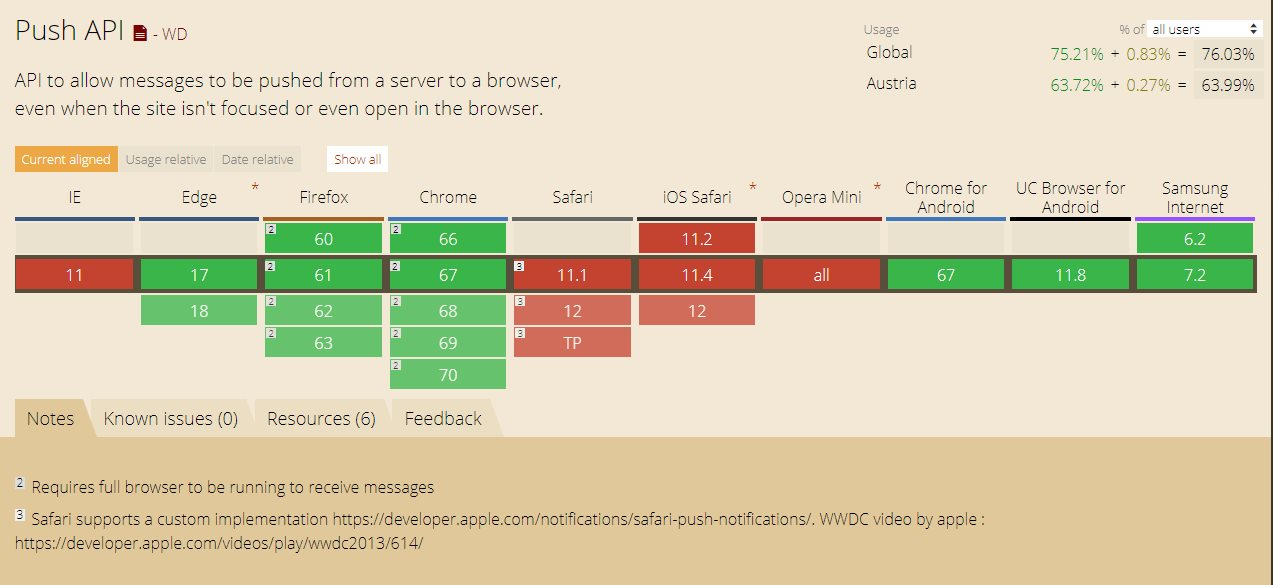
\includegraphics[width=10cm]{BilderAllgemein/BrowserPushAPI}\medskip
	\caption{Kompabilität Push Notifikation \cite{BrowserSupport}}
	\label{fig:BrowserPushAPI}
\end{figure}




\section{Geolocation API}
%https://appdevelopermagazine.com/5877/2018/3/1/progressive-web-apps-vs-native-apps:-showdown-in-2018/
Die Geolocation API kann nach Zustimmung des Benutzers den Standort bestimmen. Diese Funktion wird verwendet  um den Benutzern zusätzlichen Nutzen zu bringen, wie z.B.: Optimierung von Benutzeranfragen, bestimmen des Standortes und Backendaufnahmen von Standortdaten für Datensammlung. 
Allerdings sind bei der Verwendung der Geolocation-API zwei wichtige Punkte zu beachten:

\begin{itemize}
    \item  sollte nur verwendet werden, wenn es für den Benutzer Vorteile bringt 
	\item  Fordern einer Erlaubnis durch den Benutzer  
\end{itemize}




In der Abbildung \ref{fig:BrowserGL} sieht man die Browserkompabilität der Geolocation zum Stand Juli 2018.
\begin{figure}[H]
	\centering
	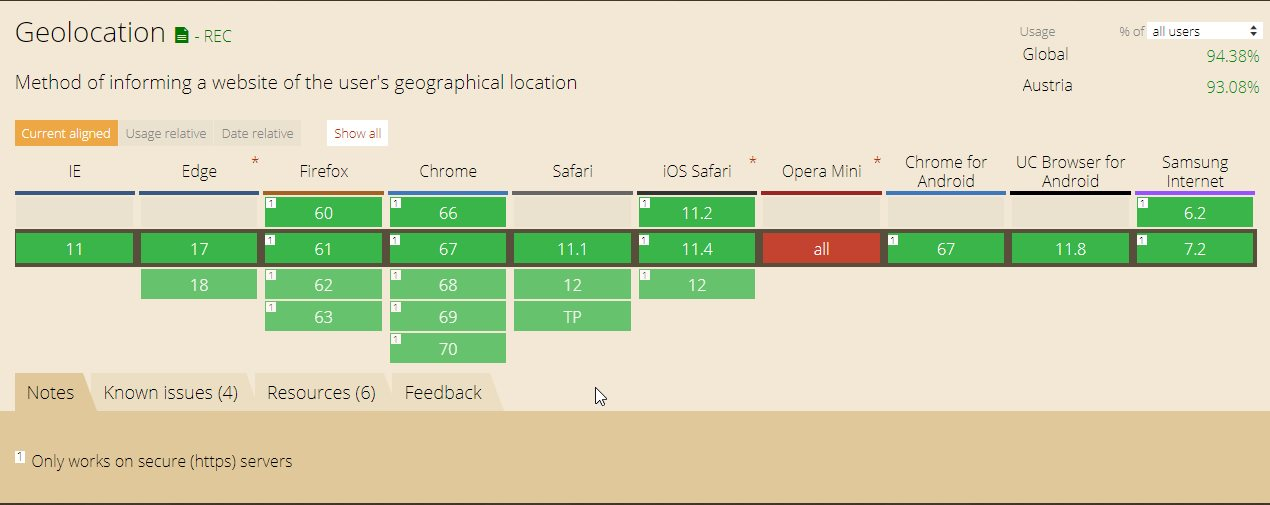
\includegraphics[width=10cm]{BilderAllgemein/BrowserGL}\medskip
	\caption{Kompabilität Geolocation \cite{BrowserSupport}}
	\label{fig:BrowserGL}
\end{figure}









